%-----------------------------------
% Kapitel 1: Einleitung
%-----------------------------------
\section{Einleitung}

Die Automatisierung des First-Level-Supports im Incident Management durch K\"unstliche Intelligenz bildet den Gegenstand der vorliegenden Arbeit. Zu kl\"aren ist, an welchen Stellen der St\"orungsbearbeitung sprachverarbeitende Modelle menschliche T\"atigkeiten \"ubernehmen k\"onnen und wo deren Grenzen liegen. Abschnitt~\ref{ausgangssituation} beschreibt hierzu die Ausgangssituation in IT-Serviceorganisationen und leitet daraus die Problemstellung ab. Abschnitt~\ref{zielsetzung} formuliert Zielsetzung und Forschungsfrage. Abschnitt~\ref{methodik} erl\"autert den methodischen Aufbau und die Vorgehensweise der Untersuchung.

\subsection{Ausgangssituation und Problemstellung}
\label{ausgangssituation}

Die betriebliche Leistungserstellung st\"utzt sich in nahezu allen Branchen auf IT-Systeme, deren Ausfall unmittelbar auf Umsatz, Lieferf\"ahigkeit und Reputation durchschl\"agt. St\"orungen des vereinbarten Servicebetriebs, im IT-Service-Management als Incidents bezeichnet, m\"ussen deshalb innerhalb zugesagter Fristen behoben werden. Erste Anlaufstelle f\"ur solche Meldungen ist der First-Level-Support, der Anfragen annimmt, erfasst, bewertet und entweder eigenst\"andig l\"ost oder an nachgelagerte Einheiten weitergibt. Seine Arbeitsqualit\"at bestimmt damit ma{\ss}geblich, wie schnell eine St\"orung \"uberhaupt der zust\"andigen Stelle zugeordnet wird.

Parallel dazu ver\"andert K\"unstliche Intelligenz (KI) die Arbeitsteilung in serviceorientierten Bereichen. Nach dem Studienbericht des Bitkom setzten 36~Prozent der deutschen Unternehmen K\"unstliche Intelligenz ein, gegen\"uber 20~Prozent im Vorjahr\footcite[Vgl.][S.~3]{Bitkom2026}. Am h\"aufigsten kommt die Technologie dabei im Kundenkontakt zum Einsatz, wo 88~Prozent der anwendenden Unternehmen sie einsetzten. Der interne IT-Support teilt mit dem externen Kundenservice die dialogbasierte Bearbeitung frei formulierter Anliegen, weshalb sich die dort erprobten Verfahren grunds\"atzlich \"ubertragen lassen; die abweichenden Rahmenbedingungen behandelt Abschnitt~\ref{voraussetzungen}\footcite[Vgl.][S.~26]{Bitkom2026}. Der Bericht weist zugleich darauf hin, dass 48~Prozent der Unternehmen hohe Anforderungen an den Datenschutz als Hindernis sehen.\footcite[Vgl.][S.~30]{Bitkom2026}

Der Handlungsdruck im First-Level-Support ergibt sich weniger aus der technologischen Verf\"ugbarkeit als aus der Struktur der Arbeit selbst. Ticketvolumina wachsen mit der Zahl betriebener Systeme und Endger\"ate, w\"ahrend ein erheblicher Teil der Bearbeitungszeit auf gleichf\"ormige T\"atigkeiten entf\"allt, etwa die Aufnahme der Meldung, ihre Zuordnung zu einer Kategorie und die Vergabe einer Priorit\"at. Fachkr\"aftemangel und Kostendruck begrenzen zugleich die M\"oglichkeit, steigende Volumina durch zus\"atzliches Personal aufzufangen.

Empirische Befunde legen nahe, dass sprachverarbeitende Modelle an dieser Stelle ansetzen k\"onnen. Brynjolfsson, Li und Raymond untersuchten den Einsatz eines auf einem Large Language Model (LLM) basierenden Assistenzsystems bei 5.172 Support-Agenten und stellten eine Zunahme der pro Stunde gel\"osten F\"alle um 15~Prozent fest, wobei unerfahrene Mitarbeitende am st\"arksten profitierten\footcite[Vgl.][S.~890]{Brynjolfsson2025}. Gartner prognostiziert dar\"uber hinaus, dass agentische KI bis 2029 80~Prozent der g\"angigen Kundenservice-Anfragen ohne menschliches Eingreifen l\"ose.\footcite[Vgl.][o.~S.]{Gartner2025}

Zwischen diesen Aussichten und dem betrieblichen Alltag besteht eine L\"ucke. Regelbasierte Chatbots sto{\ss}en bei frei formulierten St\"orungsmeldungen an Grenzen, weil ihre Entscheidungslogik auf vordefinierten Schl\"usselw\"ortern und starren Dialogpfaden beruht, wie Abschnitt~\ref{chatbotAbgrenzung} im Einzelnen darlegt. LLMs verarbeiten unstrukturierte Eingaben zuverl\"assiger, werfen aber Fragen nach der Verl\"asslichkeit generierter Ausgaben, dem Umgang mit personenbezogenen Daten und der Reichweite maschineller Entscheidungen auf. Vorliegende Beitr\"age behandeln vorrangig einzelne Anwendungsf\"alle oder die Modellebene; eine prozessorientierte Betrachtung des gesamten First-Level-Support-Prozesses fehlt weitgehend, wie die Aufarbeitung des Forschungsstands in Abschnitt~\ref{aiopsStand} zeigt. An dieser Stelle setzt die vorliegende Arbeit an, deren Zielsetzung der folgende Abschnitt pr\"azisiert.

\subsection{Zielsetzung und Forschungsfrage}
\label{zielsetzung}

Ziel ist die literaturbasierte Entwicklung eines Soll-Konzeptes f\"ur einen KI-gest\"utzten First-Level-Support-Prozess im Incident Management. Den Ausgangspunkt bildet die Analyse des Ist-Prozesses nach dem Referenzmodell der IT Infrastructure Library (ITIL), der in Business Process Model and Notation (BPMN) 2.0 modelliert wird, um Schwachstellen und Automatisierungspotenziale an konkreten Prozessschritten zu lokalisieren. Darauf aufbauend konzipiert die Arbeit einen hybriden Soll-Prozess, der LLM-gest\"utzte Prozessschritte mit menschlichen Entscheidungsknoten im Sinne eines Human-in-the-Loop verbindet und die Datenschutz-Grundverordnung (DSGVO) sowie den EU AI Act als Design-Pr\"amissen ber\"ucksichtigt. Als Ergebnis entsteht ein BPMN-modelliertes Referenzkonzept, dessen erwartete Wirkung anhand etablierter Service-Desk-Kennzahlen eingesch\"atzt wird.

Daraus leitet sich die zentrale Forschungsfrage ab:

\begin{quote}
\glqq Wie kann der First-Level-Support im Incident Management durch den Einsatz von Large Language Models prozessual automatisiert werden, sodass Effizienzpotenziale realisiert und zugleich Qualit\"ats-, Datenschutz- und Kontrollanforderungen gewahrt bleiben?\grqq{}
\end{quote}

Drei Teilfragen strukturieren die Beantwortung:

\begin{itemize}[leftmargin=3.2em,nosep]
	\item[TF1:] Wie verl\"auft der First-Level-Support-Prozess nach dem ITIL-Referenzmodell und welche Schwachstellen weist er auf?
	\item[TF2:] Wie ist ein KI-gest\"utzter Soll-Prozess zu gestalten, der Automatisierung mit menschlicher Kontrolle verbindet?
	\item[TF3:] Welche Auswirkungen auf die Prozesskennzahlen sind zu erwarten und welche Grenzen stehen einer solchen Gestaltung entgegen?
\end{itemize}

Die Untersuchung bleibt konzeptionell-literaturbasiert. Eine prototypische Implementierung des Konzeptes und dessen empirische Validierung im Unternehmenskontext sind nicht Gegenstand der Arbeit; ausgewiesen werden erwartete, nicht gemessene Wirkungen. Auf welchem methodischen Weg das Konzept entwickelt wird, erl\"autert Abschnitt~\ref{methodik}.

\subsection{Methodischer Aufbau und Vorgehensweise}
\label{methodik}

Die Arbeit folgt dem gestaltungsorientierten Paradigma der Wirtschaftsinformatik. Gegenstand ist nicht die Erkl\"arung bestehenden Verhaltens, sondern die Konstruktion und Bewertung eines Artefakts, n\"amlich des BPMN-modellierten Soll-Konzeptes f\"ur den First-Level-Support. Peffers et al.~charakterisieren die Design Science als Ansatz, der IT-Artefakte zur L\"osung erkannter organisatorischer Probleme schafft und bewertet; das Memorandum zur gestaltungsorientierten Wirtschaftsinformatik formuliert f\"ur den deutschsprachigen Raum vergleichbare Anforderungen an Abstraktion, Originalit\"at und Nutzen der entwickelten Artefakte\footcites[Vgl.][hier S.~49]{Peffers2007}[][hier S.~668]{Oesterle2010}. Das verhaltenswissenschaftliche Paradigma verfolgt demgegen\"uber ein anderes Ziel, indem es Hypothesen \"uber Wirkungszusammenh\"ange empirisch pr\"uft. Nach Wilde und Hess seien beide Ausrichtungen in der Wirtschaftsinformatik etabliert, unterschieden sich jedoch in Methodenwahl und Erkenntnisanspruch\footcite[Vgl.][hier S.~281]{WildeHess2007}. Der gestaltungsorientierte Zugang ist hier angemessen, weil die Forschungsfrage nach dem Wie einer Konstruktion fragt und nicht nach dem Ob eines Wirkungszusammenhangs. Letzteres verlangte eine empirische Hypothesenpr\"ufung, die eine bereits bestehende Implementierung voraussetzen w\"urde.

Als Vorgehensmodell dient die Design Science Research Methodology (DSRM) nach Peffers et al., die den Gestaltungsprozess in sechs Aktivit\"aten gliedert, n\"amlich Problemidentifikation, Zieldefinition, Entwurf und Entwicklung, Demonstration, Evaluation und Kommunikation\footcite[Vgl.][S.~52]{Peffers2007}. Vier dieser Aktivit\"aten pr\"agen den Aufbau der Arbeit. Die Demonstration entf\"allt, da keine prototypische Umsetzung erfolgt und damit kein Artefakt vorliegt, das auf einen konkreten Fall angewendet werden k\"onnte; die Kommunikation leistet die vorliegende Arbeit selbst. Der Aufbau der Arbeit folgt dieser Struktur. Kapitel~1 und 3 identifizieren das Problem, indem sie den Handlungsbedarf begr\"unden und den Ist-Prozess samt seiner Schwachstellen analysieren. Kapitel~2 legt die theoretische und technologische Wissensbasis. Kapitel~4 entwickelt das Artefakt, Kapitel~5 evaluiert es argumentativ, und Kapitel~6 beantwortet die Forschungsfrage. \autoref{fig:dsrm} ordnet die Kapitel den Phasen des Modells zu.

\begin{figure}[htbp]
	\centering
	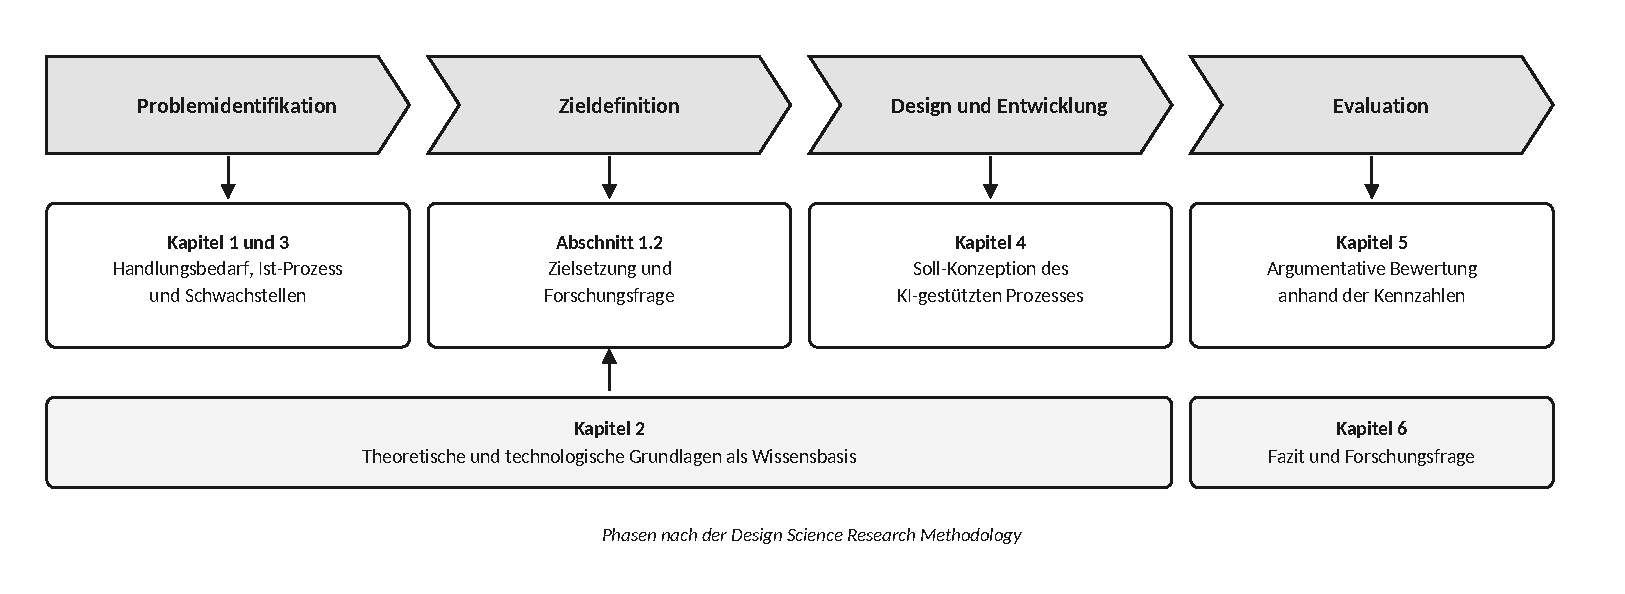
\includegraphics[width=\textwidth]{abb/abb1-dsrm.pdf}
	\caption{Aufbau der Arbeit im DSRM-Phasenmodell}
	\label{fig:dsrm}
	\par\vspace{0.4em}{\footnotesize Dargestellt sind die vier Aktivit"aten, die den Aufbau der Arbeit pr"agen; Demonstration und Kommunikation entfallen aus den oben genannten Gr"unden. Quelle: In Anlehnung an Peffers et al.~(2007), S.~52.}
\end{figure}

Die Grundlagen- und Analysekapitel st\"utzen sich auf eine strukturierte Literaturrecherche in den Datenbanken IEEE Xplore, ACM Digital Library, arXiv und SpringerLink, erg\"anzt um Standardwerke, Rahmenwerke wie ITIL~4 und BPMN~2.0, die einschl\"agigen Rechtsquellen sowie aktuelle Praxisstudien. Die Aufbereitung erfolgt konzeptzentriert nach Webster und Watson, sodass die Argumentation den Themen und nicht den einzelnen Publikationen folgt\footcite[Vgl.][hier S.~xvii]{Webster2002}. Der Suchprozess wird in Anlehnung an vom Brocke et al.~dokumentiert, um die Nachvollziehbarkeit der Quellenauswahl zu sichern; die verwendeten Suchbegriffe, Datenbanken und Auswahlkriterien weist Anhang~I aus.\footcite[Vgl.][hier S.~2211]{VomBrocke2009}

BPMN~2.0 dient als einheitliche Modellierungssprache f\"ur Ist- und Soll-Modell; die Begr\"undung dieser Methodenwahl erfolgt in Abschnitt~2.3. Da keine empirische Erhebung stattfindet, bewertet Kapitel~5 das Konzept argumentativ anhand der in Abschnitt~3.3 definierten Kennzahlen sowie anhand von Befunden der Literatur. Dieses Vorgehen erlaubt Aussagen \"uber die erwartete Wirkungsrichtung, nicht \"uber tats\"achlich erreichte Werte in einer konkreten Organisation, was die Aussagekraft der Evaluation begrenzt. Die f\"ur die Konzeption ben\"otigten Grundlagen entwickelt das folgende Kapitel.
